\documentclass[twoside]{article}

\RequirePackage[l2tabu, orthodox]{nag}
\documentclass{article}

% FONTS
\usepackage[T1]{fontenc}

% Replace default Latin Modern typewriter with its proportional counterpart
% http://www.tug.dk/FontCatalogue/lmoderntypewriterprop/
\renewcommand*\ttdefault{lmvtt}


%%% OPTION 1 - Fourier Math + New Century Schoolbook + ParaType Sans

% % Import Fourier Math (this imposes its own New Century Schoolbook type)
% % http://www.ctan.org/tex-archive/fonts/fouriernc/
%\usepackage{fouriernc}
%\usepackage{amsmath}
% % Replace with TeX Gyre Schola version of New Century Schoolbook (must scale!)
% % http://www.tug.dk/FontCatalogue/tgschola/
%\usepackage[scale=0.92]{tgschola}
%\usepackage[scaled=0.88]{PTSans}

%% OPTION 2 - MathDesign Math + Bitstream Charter + ParaType Sans

% Import MathDesign (this brings along Bitstream Charter)
% http://www.ctan.org/tex-archive/fonts/mathdesign/
\usepackage[bitstream-charter]{mathdesign}
\usepackage{amsmath}
\usepackage[scaled=0.92]{PTSans}


% %%% OPTION 3 - MTPRO 2 Math + Termes Times + ParaType Sans

% \usepackage{tgtermes}
% \usepackage{amsmath}
% \usepackage[subscriptcorrection,
%             amssymbols,
%             mtpbb,
%             mtpcal,
%             nofontinfo  % suppresses all warnings
%            ]{mtpro2}
% \usepackage{scalefnt,letltxmacro}
% \LetLtxMacro{\oldtextsc}{\textsc}
% \renewcommand{\textsc}[1]{\oldtextsc{\scalefont{1.10}#1}}
% \usepackage[scaled=0.92]{PTSans}

% GEOMETRY
\usepackage[
  paper  = letterpaper,
  left   = 1.65in,
  right  = 1.65in,
  top    = 1.0in,
  bottom = 1.0in,
  ]{geometry}

% COLOR
\usepackage[usenames,dvipsnames]{xcolor}
\definecolor{shadecolor}{gray}{0.9}

% SPACING and TEXT
\usepackage[final,expansion=alltext]{microtype}
\usepackage[english]{babel}
\usepackage[parfill]{parskip}
\usepackage{afterpage}
\usepackage{framed}
\usepackage{verbatim}

%redefine the leftbar environment to accept a width and coloring options
\renewenvironment{leftbar}[1][\hsize]
{%
  \def\FrameCommand
  {%
    {\color{Gray}\vrule width 3pt}%
    \hspace{10pt}%
    %\hspace{0pt}\fboxsep=\FrameSep\colorbox{black!10}%
  }%
  \MakeFramed{\hsize#1\advance\hsize-\width\FrameRestore}%
}%
{\endMakeFramed}

% define a paragraph header function
\DeclareRobustCommand{\parhead}[1]{\textbf{#1}~}

% EDITING
% line numbering in left margin
\usepackage{lineno}
\renewcommand\linenumberfont{\normalfont
                             \footnotesize
                             \sffamily
                             \color{SkyBlue}}
% ragged paragraphs in right margin
\usepackage{ragged2e}
\DeclareRobustCommand{\sidenote}[1]{\marginpar{
                                    \RaggedRight
                                    \textcolor{Plum}{\textsf{#1}}}}
% paragraph counter in right margin
\newcommand{\parnum}{\bfseries\P\arabic{parcount}}
\newcounter{parcount}
\newcommand\p{%
    \stepcounter{parcount}%
    \leavevmode\marginpar[\hfill\parnum]{\parnum}%
}
% paragraph helper
%\DeclareRobustCommand{\PP}{\textcolor{Plum}{\P} }

% COUNTERS
\renewcommand{\labelenumi}{\color{black!67}{\arabic{enumi}.}}
\renewcommand{\labelenumii}{{\color{black!67}(\alph{enumii})}}
\renewcommand{\labelitemi}{{\color{black!67}\textbullet}}

% FIGURES
\usepackage{graphicx}
\usepackage[labelfont=bf]{caption}
\usepackage[format=hang]{subcaption}

% TABLES
\usepackage{booktabs}

% ALGORITHMS
\usepackage[algoruled]{algorithm2e}
\usepackage{listings}
\usepackage{fancyvrb}
\fvset{fontsize=\normalsize}

% BIBLIOGRAPHY
\usepackage{natbib}

% HYPERREF
\usepackage[colorlinks,linktoc=all]{hyperref}
\usepackage[all]{hypcap}
\hypersetup{citecolor=BurntOrange}
\hypersetup{linkcolor=MidnightBlue}
\hypersetup{urlcolor=MidnightBlue}

% CLEVEREF must come after HYPERREF
\usepackage[nameinlink]{cleveref}

% ACRONYMS
\usepackage[acronym,smallcaps,nowarn]{glossaries}
% \makeglossaries

% COLOR DEFINITIONS
\newcommand{\red}[1]{\textcolor{BrickRed}{#1}}
\newcommand{\orange}[1]{\textcolor{BurntOrange}{#1}}
\newcommand{\green}[1]{\textcolor{OliveGreen}{#1}}
\newcommand{\blue}[1]{\textcolor{MidnightBlue}{#1}}
\newcommand{\gray}[1]{\textcolor{black!60}{#1}}

% LISTINGS DEFINTIONS
\lstdefinestyle{mystyle}{
    commentstyle=\color{OliveGreen},
    keywordstyle=\color{BurntOrange},
    numberstyle=\tiny\color{black!60},
    stringstyle=\color{MidnightBlue},
    basicstyle=\ttfamily,
    breakatwhitespace=false,
    breaklines=true,
    captionpos=b,
    keepspaces=true,
    numbers=left,
    numbersep=5pt,
    showspaces=false,
    showstringspaces=false,
    showtabs=false,
    tabsize=2
}
\lstset{style=mystyle}

\DeclareRobustCommand{\mb}[1]{\ensuremath{\boldsymbol{\mathbf{#1}}}}
\DeclareRobustCommand{\KL}[2]{\ensuremath{\textrm{KL}\left(#1\;\|\;#2\right)}}

\newcommand{\supp}{\textrm{supp}}

\newcommand{\E}{\mathbb{E}}
\newcommand{\Var}{\mathbb{V}\textrm{ar}}

% Redundant with reals, naturals, below
\newcommand{\bbN}{\mathbb{N}}
\newcommand{\bbZ}{\mathbb{Z}}
\newcommand{\bbR}{\mathbb{R}}
\newcommand{\bbS}{\mathbb{S}}
\newcommand{\bbH}{\mathbb{H}}


\newcommand{\bA}{\boldsymbol{A}}
\newcommand{\bB}{\boldsymbol{B}}
\newcommand{\bC}{\boldsymbol{C}}
\newcommand{\bD}{\boldsymbol{D}}
\newcommand{\bE}{\boldsymbol{E}}
\newcommand{\bF}{\boldsymbol{F}}
\newcommand{\bG}{\boldsymbol{G}}
\newcommand{\bH}{\boldsymbol{H}}
\newcommand{\bI}{\boldsymbol{I}}
\newcommand{\bJ}{\boldsymbol{J}}
\newcommand{\bK}{\boldsymbol{K}}
\newcommand{\bL}{\boldsymbol{L}}
\newcommand{\bM}{\boldsymbol{M}}
\newcommand{\bN}{\boldsymbol{N}}
\newcommand{\bO}{\boldsymbol{O}}
\newcommand{\bP}{\boldsymbol{P}}
\newcommand{\bQ}{\boldsymbol{Q}}
\newcommand{\bR}{\boldsymbol{R}}
\newcommand{\bS}{\boldsymbol{S}}
\newcommand{\bT}{\boldsymbol{T}}
\newcommand{\bU}{\boldsymbol{U}}
\newcommand{\bV}{\boldsymbol{V}}
\newcommand{\bW}{\boldsymbol{W}}
\newcommand{\bX}{\boldsymbol{X}}
\newcommand{\bY}{\boldsymbol{Y}}
\newcommand{\bZ}{\boldsymbol{Z}}
\newcommand{\ba}{\boldsymbol{a}}
\newcommand{\bb}{\boldsymbol{b}}
\newcommand{\bc}{\boldsymbol{c}}
\newcommand{\bd}{\boldsymbol{d}}
\newcommand{\be}{\boldsymbol{e}}
\newcommand{\bbf}{\boldsymbol{f}}
\newcommand{\bg}{\boldsymbol{g}}
\newcommand{\bh}{\boldsymbol{h}}
\newcommand{\bi}{\boldsymbol{i}}
\newcommand{\bj}{\boldsymbol{j}}
\newcommand{\bk}{\boldsymbol{k}}
\newcommand{\bl}{\boldsymbol{l}}
\newcommand{\bbm}{\boldsymbol{m}}
\newcommand{\bn}{\boldsymbol{n}}
\newcommand{\bo}{\boldsymbol{o}}
\newcommand{\bp}{\boldsymbol{p}}
\newcommand{\bq}{\boldsymbol{q}}
\newcommand{\br}{\boldsymbol{r}}
\newcommand{\bs}{\boldsymbol{s}}
\newcommand{\bt}{\boldsymbol{t}}
\newcommand{\bu}{\boldsymbol{u}}
\newcommand{\bv}{\boldsymbol{v}}
\newcommand{\bw}{\boldsymbol{w}}
\newcommand{\bx}{\boldsymbol{x}}
\newcommand{\by}{\boldsymbol{y}}
\newcommand{\bz}{\boldsymbol{z}}

\newcommand{\balpha}{\boldsymbol{\alpha}}
\newcommand{\bbeta}{\boldsymbol{\beta}}
\newcommand{\boldeta}{\boldsymbol{\eta}}
\newcommand{\bkappa}{\boldsymbol{\kappa}}
\newcommand{\bgamma}{\boldsymbol{\gamma}}
\newcommand{\blambda}{\boldsymbol{\lambda}}
\newcommand{\bmu}{\boldsymbol{\mu}}
\newcommand{\bnu}{\boldsymbol{\nu}}
\newcommand{\brho}{\boldsymbol{\rho}}
\newcommand{\bphi}{\boldsymbol{\phi}}
\newcommand{\bpi}{\boldsymbol{\pi}}
\newcommand{\bpsi}{\boldsymbol{\psi}}
\newcommand{\bsigma}{\boldsymbol{\sigma}}
\newcommand{\btheta}{\boldsymbol{\theta}}
\newcommand{\bomega}{\boldsymbol{\omega}}
\newcommand{\bxi}{\boldsymbol{\xi}}
\newcommand{\bGamma}{\boldsymbol{\Gamma}}
\newcommand{\bLambda}{\boldsymbol{\Lambda}}
\newcommand{\bOmega}{\boldsymbol{\Omega}}
\newcommand{\bPhi}{\boldsymbol{\Phi}}
\newcommand{\bPi}{\boldsymbol{\Pi}}
\newcommand{\bPsi}{\boldsymbol{\Psi}}
\newcommand{\bSigma}{\boldsymbol{\Sigma}}
\newcommand{\bTheta}{\boldsymbol{\Theta}}
\newcommand{\bUpsilon}{\boldsymbol{\Upsilon}}
\newcommand{\bXi}{\boldsymbol{\Xi}}
\newcommand{\bepsilon}{\boldsymbol{\epsilon}}

\newcommand{\mcA}{\mathcal{A}}
\newcommand{\mcB}{\mathcal{B}}
\newcommand{\mcC}{\mathcal{C}}
\newcommand{\mcD}{\mathcal{D}}
\newcommand{\mcE}{\mathcal{E}}
\newcommand{\mcF}{\mathcal{F}}
\newcommand{\mcG}{\mathcal{G}}
\newcommand{\mcH}{\mathcal{H}}
\newcommand{\mcI}{\mathcal{I}}
\newcommand{\mcJ}{\mathcal{J}}
\newcommand{\mcK}{\mathcal{K}}
\newcommand{\mcL}{\mathcal{L}}
\newcommand{\mcM}{\mathcal{M}}
\newcommand{\mcN}{\mathcal{N}}
\newcommand{\mcO}{\mathcal{O}}
\newcommand{\mcP}{\mathcal{P}}
\newcommand{\mcQ}{\mathcal{Q}}
\newcommand{\mcR}{\mathcal{R}}
\newcommand{\mcS}{\mathcal{S}}
\newcommand{\mcT}{\mathcal{T}}
\newcommand{\mcU}{\mathcal{U}}
\newcommand{\mcV}{\mathcal{V}}
\newcommand{\mcW}{\mathcal{W}}
\newcommand{\mcX}{\mathcal{X}}
\newcommand{\mcY}{\mathcal{Y}}
\newcommand{\mcZ}{\mathcal{Z}}

\newcommand{\trans}{\mathsf{T}}
\newcommand{\naturals}{\mathbb{N}}
\newcommand{\reals}{\mathbb{R}}
\def\argmax{\operatornamewithlimits{arg\,max}}
\def\argmin{\operatornamewithlimits{arg\,min}}

\newcommand{\distNormal}{\mathcal{N}}
\newcommand{\distGamma}{\mathrm{Gamma}}
\newcommand{\distBernoulli}{\mathrm{Bern}}
\newcommand{\distBinomial}{\mathrm{Bin}}
\newcommand{\distCategorical}{\mathrm{Cat}}
\newcommand{\distDirichlet}{\mathrm{Dir}}
\newcommand{\distMultinomial}{\mathrm{Mult}}
\newcommand{\distPolyaGamma}{\mathrm{PG}}
\newcommand{\distMNIW}{\mathrm{MNIW}}
\newcommand{\distBeta}{\mathrm{Beta}}

\newcommand{\prt}[1]{\frac{\partial}{\partial #1}}
\newcommand{\deriv}[1]{\frac{\mathrm{d}}{\mathrm{d} #1}}


\newcommand{\TODO}[1]{\textcolor{red}{[TODO: #1]}}

\newcommand{\bbI}{\mathbb{I}}
\newcommand{\bbE}{\mathbb{E}}
\newcommand{\bone}{\boldsymbol{1}}
\newcommand{\bigO}{\mathcal{O}}
\newcommand{\iid}[1]{\stackrel{\text{iid}}{#1}}
\newcommand\indep{\protect\mathpalette{\protect\independenT}{\perp}}
\def\independenT#1#2{\mathrel{\rlap{$#1#2$}\mkern4mu{#1#2}}}
\DeclareMathOperator{\Skew}{Skew}
\DeclareMathOperator{\Symm}{Sym}
\DeclareMathOperator{\tr}{tr}

%\DeclareMathOperator{\KL}{KL}
\newcommand{\given}{\, | \,}

\DeclareMathOperator{\diag}{diag}
\let\vec\relax% Set equal to \relax so that LaTeX thinks it's not defined
\DeclareMathOperator{\vec}{vec}
\let\Re\relax
\DeclareMathOperator{\Re}{\textup{Re}}
\let\Im\relax
\DeclareMathOperator{\Im}{\textup{Im}}

% Backcompat: dif and diff both work
\newcommand*\dif{\mathop{}\!\mathrm{d}}
\newcommand*\diff{\mathop{}\!\mathrm{d}}


% !TEX root = template.tex

\newacronym{KL}{kl}{Kullback-Leibler}
\newacronym{ELBO}{elbo}{evidence lower bound}
\newacronym{SVI}{svi}{stochastic variational inference}
\newacronym{GMM}{gmm}{Gaussian mixture model}
\newacronym{LDA}{lda}{latent Dirichlet allocation}



\usepackage{blindtext}

\usepackage{aistats2018}

\DeclareRobustCommand{\parhead}[1]{\textbf{#1}~}

% If your paper is accepted, change the options for the package
% aistats2018 as follows:
%
%\usepackage[accepted]{aistats2018}
%
% This option will print headings for the title of your paper and
% headings for the authors names, plus a copyright note at the end of
% the first column of the first page.


\begin{document}

% If your paper is accepted and the title of your paper is very long,
% the style will print as headings an error message. Use the following
% command to supply a shorter title of your paper so that it can be
% used as headings.
%
%\runningtitle{I use this title instead because the last one was very long}

% If your paper is accepted and the number of authors is large, the
% style will print as headings an error message. Use the following
% command to supply a shorter version of the authors names so that
% they can be used as headings (for example, use only the surnames)
%
%\runningauthor{Surname 1, Surname 2, Surname 3, ...., Surname n}

\twocolumn[

\aistatstitle{Reparameterizing the Birkhoff Polytope for \\
  Variational Permutation Inference: Supplementary Material}

% \aistatsauthor{ Gonzalo E. Mena$^*$ \And Scott W. Linderman$^*$
%   \And  Hal Cooper \AND Liam Paninski \And John P. Cunningham }

% \aistatsaddress{ Columbia University}

\aistatsauthor{ Anonymous Authors }

\aistatsaddress{ Anonymous Institutions}
]
\appendix



\section{Alternative methods of discrete variational inference}

Recently there have been a number of proposals for extending the
reparameterization trick~\citep{rezende2014stochastic, Kingma2014} to
high dimensional discrete problems\footnote{Discrete inference is only
  problematic in the high dimensional case, since in low dimensional
  problems we can enumerate the possible values of~$x$ and compute the
  normalizing constant~$p(y) = \sum_x p(y, x)$.} by relaxing them to
analogous continuous problems \citep{maddison2016concrete,
  jang2016categorical, kusner2016gans}.  These approaches are based on
the following observation: if~$x \in \{0,1\}^N$ is a one-hot vector
drawn from a categorical distribution, then the support of~$p(x)$ is
the set of vertices of the~$N-1$ dimensional simplex.  We can
represent the distribution of~$x$ as an atomic density on the simplex.

\subsection{The Gumbel-softmax method}
Viewing~$x$ as a vertex of the simplex motivates a natural relaxation:
rather than restricting ourselves to atomic measures,
consider continuous densities on the simplex. To be concrete, suppose
the density of~$x$ is defined by the transformation,
\begin{align*}
  \xi_n &\iid{\sim} \mathrm{Gumbel}(0, 1) \\
  \psi_n & = \log \theta_n + \xi_n  \\
  x &=  \mathsf{softmax}(\psi / \tau) \\
        &=\left(\frac{e^{\psi_1 / \tau}}{\sum_{n=1}^N e^{\psi_n / \tau}},
      \,\ldots,\,
      \frac{e^{\psi_N / \tau}}{\sum_{n=1}^N e^{\psi_n / \tau}} \right).
\end{align*}
The output~$x$ is now a point on the simplex, and the
parameter~${\theta = (\theta_1, \ldots, \theta_N)}$ can be optimized
via stochastic gradient ascent with the reparameterization trick.

The Gumbel distribution leads to a nicely interpretable model:
when~$\theta$ is a probability mass function, adding Gumbel noise and
taking the argmax yields an exact sample from~$\theta$; the softmax is
a natural relaxation. As the temperature~$\tau$ goes to zero, the
softmax converges to the argmax function. Ultimately, however, this is
just a continuous relaxation of an atomic density to a continuous
density.

Stick-breaking and rounding offer two alternative ways of conceiving a
relaxed version of a discrete random variable, and both are amenable
to reparameterization. However, unlike the Gumbel-Softmax, these
relaxations enable extensions to more complex combinatorial objects,
notably, permutations.

\subsection{Stick-breaking}

The stick-breaking transformation to the Birkhoff polytope presented
in the main text contains a recipe for stick-breaking on the simplex.
In particular, as we filled in the first row of the doubly-stochastic
matrix, we were transforming a real-valued vector~$\psi \in \reals^{N-1}$
to a point in the simplex.  We present this procedure for
discrete variational inference again here in simplified form.
Start with a reparameterization of a Gaussian vector,
\begin{align*}
  \xi_n &\iid{\sim} \distNormal(0, 1), \\
  \psi_n & = \mu_n + \eta_n \xi_n, \qquad 1 \leq n \leq N-1,
\end{align*}
parameterized by~${\theta = (\mu_n, \eta_n)_{n=1}^{N-1}}$. 
Then map this to a point in the simplex:
\begin{align*}
  x_1 &= \sigma(\psi_1 / \tau), \\
  x_n &= \sigma(\psi_n / \tau) \left(1- \sum_{m=1}^{n-1} x_m\right), \qquad 2 \leq n \leq N-1,  \\
  x_N &= 1- \sum_{m=1}^{N-1} x_m,
\end{align*}
where~${\sigma(u) = (1+e^{-u})^{-1}}$ is the logistic
function. Here,~$\sigma(\psi_n/\tau)$ is the fraction of the remaining
``stick'' of probability mass assigned to~$x_n$.  This procedure is
invertible, the Jacobian~$\frac{\mathrm{d}x}{\mathrm{d}\psi}$ is
lower-triangular, and the determinant of the Jacobian is easy to
compute.  \citet{linderman2015dependent} compute the density of~$x$
implied by a Gaussian density on~$\psi$.

The temperature~$\tau$ controls how concentrated $p(\pi)$ is at the
vertices of the simplex, and with appropriate choices of parameters,
in the limit ~$\tau \to 0$ we can recover any categorial
distribution. In the other limit, as ~$\tau \to \infty$, the density
concentrates on a point in the interior of the simplex determined by
the parameters, and for intermediate values, the density is continuous
on the simplex.

Finally, note that the logistic-normal construction only one possible
choice.  We could instead
let~${\psi_n \sim \mathrm{Beta}(\tfrac{a_n}{\tau}, \tfrac{b_n}{\tau})}$
and~${x_n = \psi_n}$. This would lead to the Dirichlet distribution on
the simplex.  The beta distribution is slightly harder to
reparameterize since it is typically simulated with a rejection
sampling procedure, but~\citet{naesseth2017reparameterization} have
shown how this can be handled with a mix of reparameterization and
score-function gradients.  Alternatively, the beta distribution could
be replaced with the Kumaraswamy distribution, which is quite similar
to the beta distribution but is easily reparameterizable.

\subsection{Rounding}
Rounding transformations also have a natural analog for discrete
variational inference.  Define the rounding operator,
\begin{align*}
  \mathsf{round}(\psi)
  &= \argmin_{e_n} \| e_n - \psi \|^2,
\end{align*}
which maps~${\psi \in \reals^N}$ to the one-hot vectors~${e_n}$;
i.e. the vectors in~${\{0,1\}^N}$ with~$n$-th entry equal to one and
all other entries equal zero.  This is equivalent to
defining~${\mathsf{round}(\psi) = e_{n^*}}$ where
\begin{align*}
  n^* &= \argmin_{n} \|e_n - \psi \|^2 \\
  &= \argmin_{n} \sum_{m \neq n} \psi_m^2 + (1 - \psi_n)^2  \\
  &= \argmin_{n} \sum_{m \neq n} \psi_m^2 + \psi_n^2 - 2\psi_n + 1 \\
  &= \argmin_{n} \|\psi\|^2 - 2\psi_n + 1 \\
  &= \argmax_n \psi_n.
\end{align*}
In the case of a tie, let~$n^*$ be the smallest index~$n$ such
that~$\psi_n > \psi_m$ for all~$m < n$. Rounding effectively
partitions the space into~$N$ disjoint ``Voronoi'' cells,
\begin{align*}
  V_n &= \Big \{ \psi \in \reals^N : \,
        \psi_n \geq \psi_m \, \forall m \; \wedge \;
        \psi_n > \psi_m \, \forall m < n
        \Big \}.
\end{align*}
By definition,~${\mathsf{round}(\psi) = e_{n^*}}$ for
all~${\psi \in V_{n^*}}$


We define a map that pulls points toward their rounded values,
\begin{align}
  \label{eq:round}
  x &=  \tau \psi + (1-\tau) \mathsf{round}(\psi).
\end{align}

\begin{proposition}
  \label{prop:round}
  For~${\tau \in [0,1]}$, the map defined by~\eqref{eq:round} moves
  points strictly closer to their rounded values so
  that~$\mathsf{round}(\psi) = \mathsf{round}(x)$.
\end{proposition}

\begin{proof}
  Note that the Voronoi cells are intersections of halfspaces
  and, as such, are convex sets.  Since~$x$ is a convex combination
  of~$\psi$ and~$e_{n^*}$, both of which belong to the convex
  set~$V_{n^*}$, $x$~must belong to~$V_{n^*}$ as well.
\end{proof}

Similarly,~$x$ will be a point on the simplex if an only if~$\psi$ is
on the simplex as well.  By analogy to the rounding transformations
for permutation inference, in categorical inference we use a Gaussian
distribution~${\psi \sim \distNormal(\mathsf{proj}(m), H)}$,
where~$\mathsf{proj}(m)$ is the projection of~$m \in \reals_+^N$ onto
the simplex.  Still, the simplex has zero measure under the Gaussian
distribution.  It follows that the rounded points~$x$ will almost
surely not be on the simplex either.  The supposition of this approach
is that this is not a problem: relaxing to the simplex is nice but not
required.

In the zero-temperature limit we obtain a discrete distribution on the
vertices of the simplex.  For~${\tau \in (0,1]}$ we have a
distribution on~${\mcX_\tau \subseteq \reals^N}$, the subset of the
reals to which the rounding operation maps. (For~${0 \leq \tau < 1}$
this is a strict subset of~$\reals^N$.) To derive the
density~$q(x)$, we need the inverse transformation and the
determinant of its Jacobian.  From Proposition~\ref{prop:round}, it
follows that the inverse transformation is given by,
\begin{align*}
  \psi &= \frac{1}{\tau} x - \frac{1 - \tau}{\tau} \mathsf{round}(x).
\end{align*}
As long as~$\psi$ is in the interior of its Voronoi cell,
the~$\mathsf{round}$ function is piecewise constant and the
Jacobian is~${\tfrac{\mathrm{d}\psi}{\mathrm{d}x} = \tfrac{1}{\tau} I}$,
and its determinant is~$\tau^{-N}$. Taken together, we have,
\begin{multline*}
  q(x; m, H) =  \\
  \tau^{-N} \distNormal \left(\frac{1}{\tau}x - \frac{1-\tau}{\tau} \mathsf{round}(x); \, \mathsf{proj}(m), H \right) \\
  \times \bbI[x \in \mcX_\tau].
\end{multline*}
Compare this to the density of the rounded random variables for
permutation inference. 

\section{Limit analysis for stick-breaking}

We show that stick-breaking for discrete variational inference can
converge to any categorical distribution in the zero-temperature
limit.  We do so with a sequence of propositions: first we show that
in the zero-temperature limit, the distribution
of~${\sigma(\psi_n / \tau)}$ converges to a Bernoulli distribution.
The we show that when~$\sigma(\psi_n / \tau)$ is Bernoulli (rather
than a continuous density on the unit interval), the distribution
on~$x$ obtained by applying the stick-breaking transformation
to~$\psi$ is categorical.

\begin{proposition}
  \label{prop:bernoulli}
  Let~${z=\sigma(\psi / \tau)}$
  with~${\psi\sim\mathcal{N}(\mu,\eta^2)}$.  In the
  limit~${\tau \to
    0}$ we have~${z \sim \distBernoulli(\Phi(-\tfrac{\mu}{\eta}))}$,
  where~$\Phi(\cdot)$ denotes the Gaussian cumulative distribution
  function (cdf). 
\end{proposition}

\begin{proof}
  Let~$F_z$ be the cdf of the random variable~$z$. Since~$z$ is a random
  variable on the unit interval, $F_z$ is a non-decreasing function
  on~$[0,1]$ with~${F_z(0)=0}$ and~${F_z(1)=1}$.
  Reparameterize~${\psi = \mu + \eta \xi}$
  where~${\xi \sim \distNormal(0,1)}$. Then we have,
  \begin{align*}
    F_z(u) &= \Pr(\sigma(\psi / \tau) < u) \\
         &= \Pr(\psi < \tau \sigma^{-1}(u)) \\
         &= \Pr(\xi < \tfrac{\tau}{\eta} \sigma^{-1}(u) - \tfrac{\mu}{\eta}))\\
         &= \Phi(-\tfrac{\tau}{\eta}\sigma^{-1}(u) - \tfrac{\mu}{\eta}).
  \end{align*}
  By the continuity of~$\Phi$ we have,
  \begin{align*}
    \lim_{\tau \to 0} F_z(u) &= \Phi(-\tfrac{\mu}{\eta}) &
    \text{for } u &\in (0,1).
  \end{align*}
  This is the cdf of a Bernoulli random with
  probability~${\rho = \Phi(-\tfrac{\mu}{\eta})}$.
\end{proof}

\begin{proposition}
  \label{prop:categorical}
  As above, let~${z_n=\sigma(\psi_n / \tau)}$.
  When~${z_n \sim \distBernoulli(\rho_n)}$
  with~${\rho_n \in [0,1]}$ for~${n=1, \ldots, N}$, the random
  variable~$x$ obtained from applying the stick-breaking
  transformation to~$z$ will have an atomic distribution with atoms
  in the vertices of $\Delta_{N}$; i.e,
  ${x \sim \distCategorical(\pi)}$ where
  \begin{align*}
    \pi_1 &= \rho_1 \\
    \pi_n &=  \rho_n \prod_{m=1}^{n-1} (1-\rho_m)  \qquad
          n=2, \ldots, N-1, \\
    \pi_N &= \prod_{m=1}^{N-1} (1-\rho_m).
\end{align*}
\end{proposition}

\begin{proof}
  From the stick-breaking definition,~${x_1 = z_1}$,
  ${x_n = z_n (1- \sum_{m < n} x_m)}$,
  and~${x_N = 1-\sum_{m < N} x_m}$.
  When~${z_n \in \{0,1\}}$ for all~${n = 1, \ldots, N-1}$,
  we have the following equivalencies. For the first element,
  \begin{align*}
    x_1 = 1 &\iff z_1 = 1;
  \end{align*}
  for~${1 < n < N-1}:$
  \begin{align*}
    x_n = 1 &\iff (z_n = 1) \bigwedge_{m=1}^{n-1} (z_m = 0);
  \end{align*}
  and for the last element,
  \begin{align*}
    x_N = 1 &\iff \bigwedge_{m=1}^{N-1} (z_m = 0).
  \end{align*}
  These events are mutually exclusive, implying that~$x$ will
  necessarily be a one-hot vector, i.e. a categorical random variable.
  Since~$z_1, \ldots, z_{N-1}$ are independent Bernoulli random
  variables, the probabilities of these events are given
  by the~${\pi, \ldots, \pi_N}$ stated in the proposition. 
\end{proof}

These two propositions, combined with the invertibility of the
stick-breaking procedure, lead to our main result.

\begin{lemma}
  In the zero-temperature limit, stick-breaking of logistic-normal
  random variables can realize any categorical distribution on~$x$.
\end{lemma}

\begin{proof}
  There is a one-to-one correspondence between~${\pi \in \Delta_N}$
  and~${\rho \in [0,1]^{N-1}}$.  Specifically,
  \begin{align*}
    \rho_1 &= \pi_1 \\
    \rho_n &= \frac{\pi_n}{\prod_{m=1}^{n=1} 1-\rho_m}
             \quad \text{for } n = 2, \ldots, N-1.
  \end{align*}
  Since these are recursively defined, we can substitute the definition
  of~$\rho_m$ to obtain an expression for~$\rho_n$ in terms of~$\pi$ only.
  Thus, by Proposition~\ref{prop:categorical}, any desired categorical
  distribution~$\pi$ implies a set of Bernoulli parameters~$\rho$.
  From Proposition~\ref{prop:bernoulli}, in the zero temperature limit,
  any desired~$\rho_n$ can be obtained with appropriate choice of
  Gaussian mean~$\mu_n$ and variance~$\eta_n^2$. Thus, stick-breaking
  can realize any categorical distribution when~${\tau \to 0}$.
\end{proof}


\section{Variational Autoencoders (VAE) with categorical latent variables}



We considered the density estimation task on MNIST digits, as in
\cite{maddison2016concrete, jang2016categorical}, where observed
digits are reconstructed from a latent discrete code. We used the
continuous ELBO for training, and evaluated performance based on the
marginal likelihood, estimated through the multi-sample variational
objective of the discretized model. We compared against the methods of
\cite{jang2016categorical, maddison2016concrete} and obtained the
results in Table~\ref{tab:vae}.  While stick-breaking and rounding
fare slightly worse than the Gumbel-softmax method, they are readily
extensible to more complex discrete objects, as shown in the main
paper.

\begin{table}[h]
  \caption{Summary of results in VAE}
  \label{tab:vae}
  \centering
  \begin{tabular}{ll}
    \textbf{Method} & $- \log p(x)$ \\
    \hline
    Gumbel-Softmax    & 106.7 \\
    Concrete  &  111.5\\
    Rounding &  121.1 \\
    Stick-breaking & 119. 8\\
    \bottomrule
  \end{tabular}
\end{table}


% \begin{table*}[t]
%   \caption{Battacharya distances in the synthetic matching experiment}
%   \label{sample-table}
%   \centering
%   \begin{tabular}{llllllll}
%    & \multicolumn{1}{c}{Rounding} & \multicolumn{1}{c}{Stick-breaking} & \multicolumn{5}{c}{Mallows}\\
%     \cmidrule(lr){2-2} \cmidrule(lr){3-3} \cmidrule(lr){4-8}
%     &    & &   $\theta=0.1$ &  $\theta=1$ & $\theta=2$ & $\theta=5$ & $\theta=10$ \\
%     \midrule
%     $\sigma=0.1$     & .06 & .09  &.93 &.51& .23  & .08 &.08\\
%     $\sigma=0.25$     & .21 & .23 & .92 &.53 & .33&  .27 &.27\\
%      $\sigma=0.5$     & .32 & .41 & .89 &.61 & .53&  .54& .54\\
%      $\sigma=0.75$     & .38   & .55 & .85 &.71 & .69&  .72 &.72\\
   
%     \bottomrule
%   \end{tabular}
% \end{table*}

Figure~\ref{fig:VAE} shows MNIST reconstructions using Gumbel-Softmax,
stick-breaking and rounding reparameterizations. In all the three
cases reconstructions are reasonably accurate, and there is diversity
in reconstructions.
\begin{figure*}[t]
  \centering
  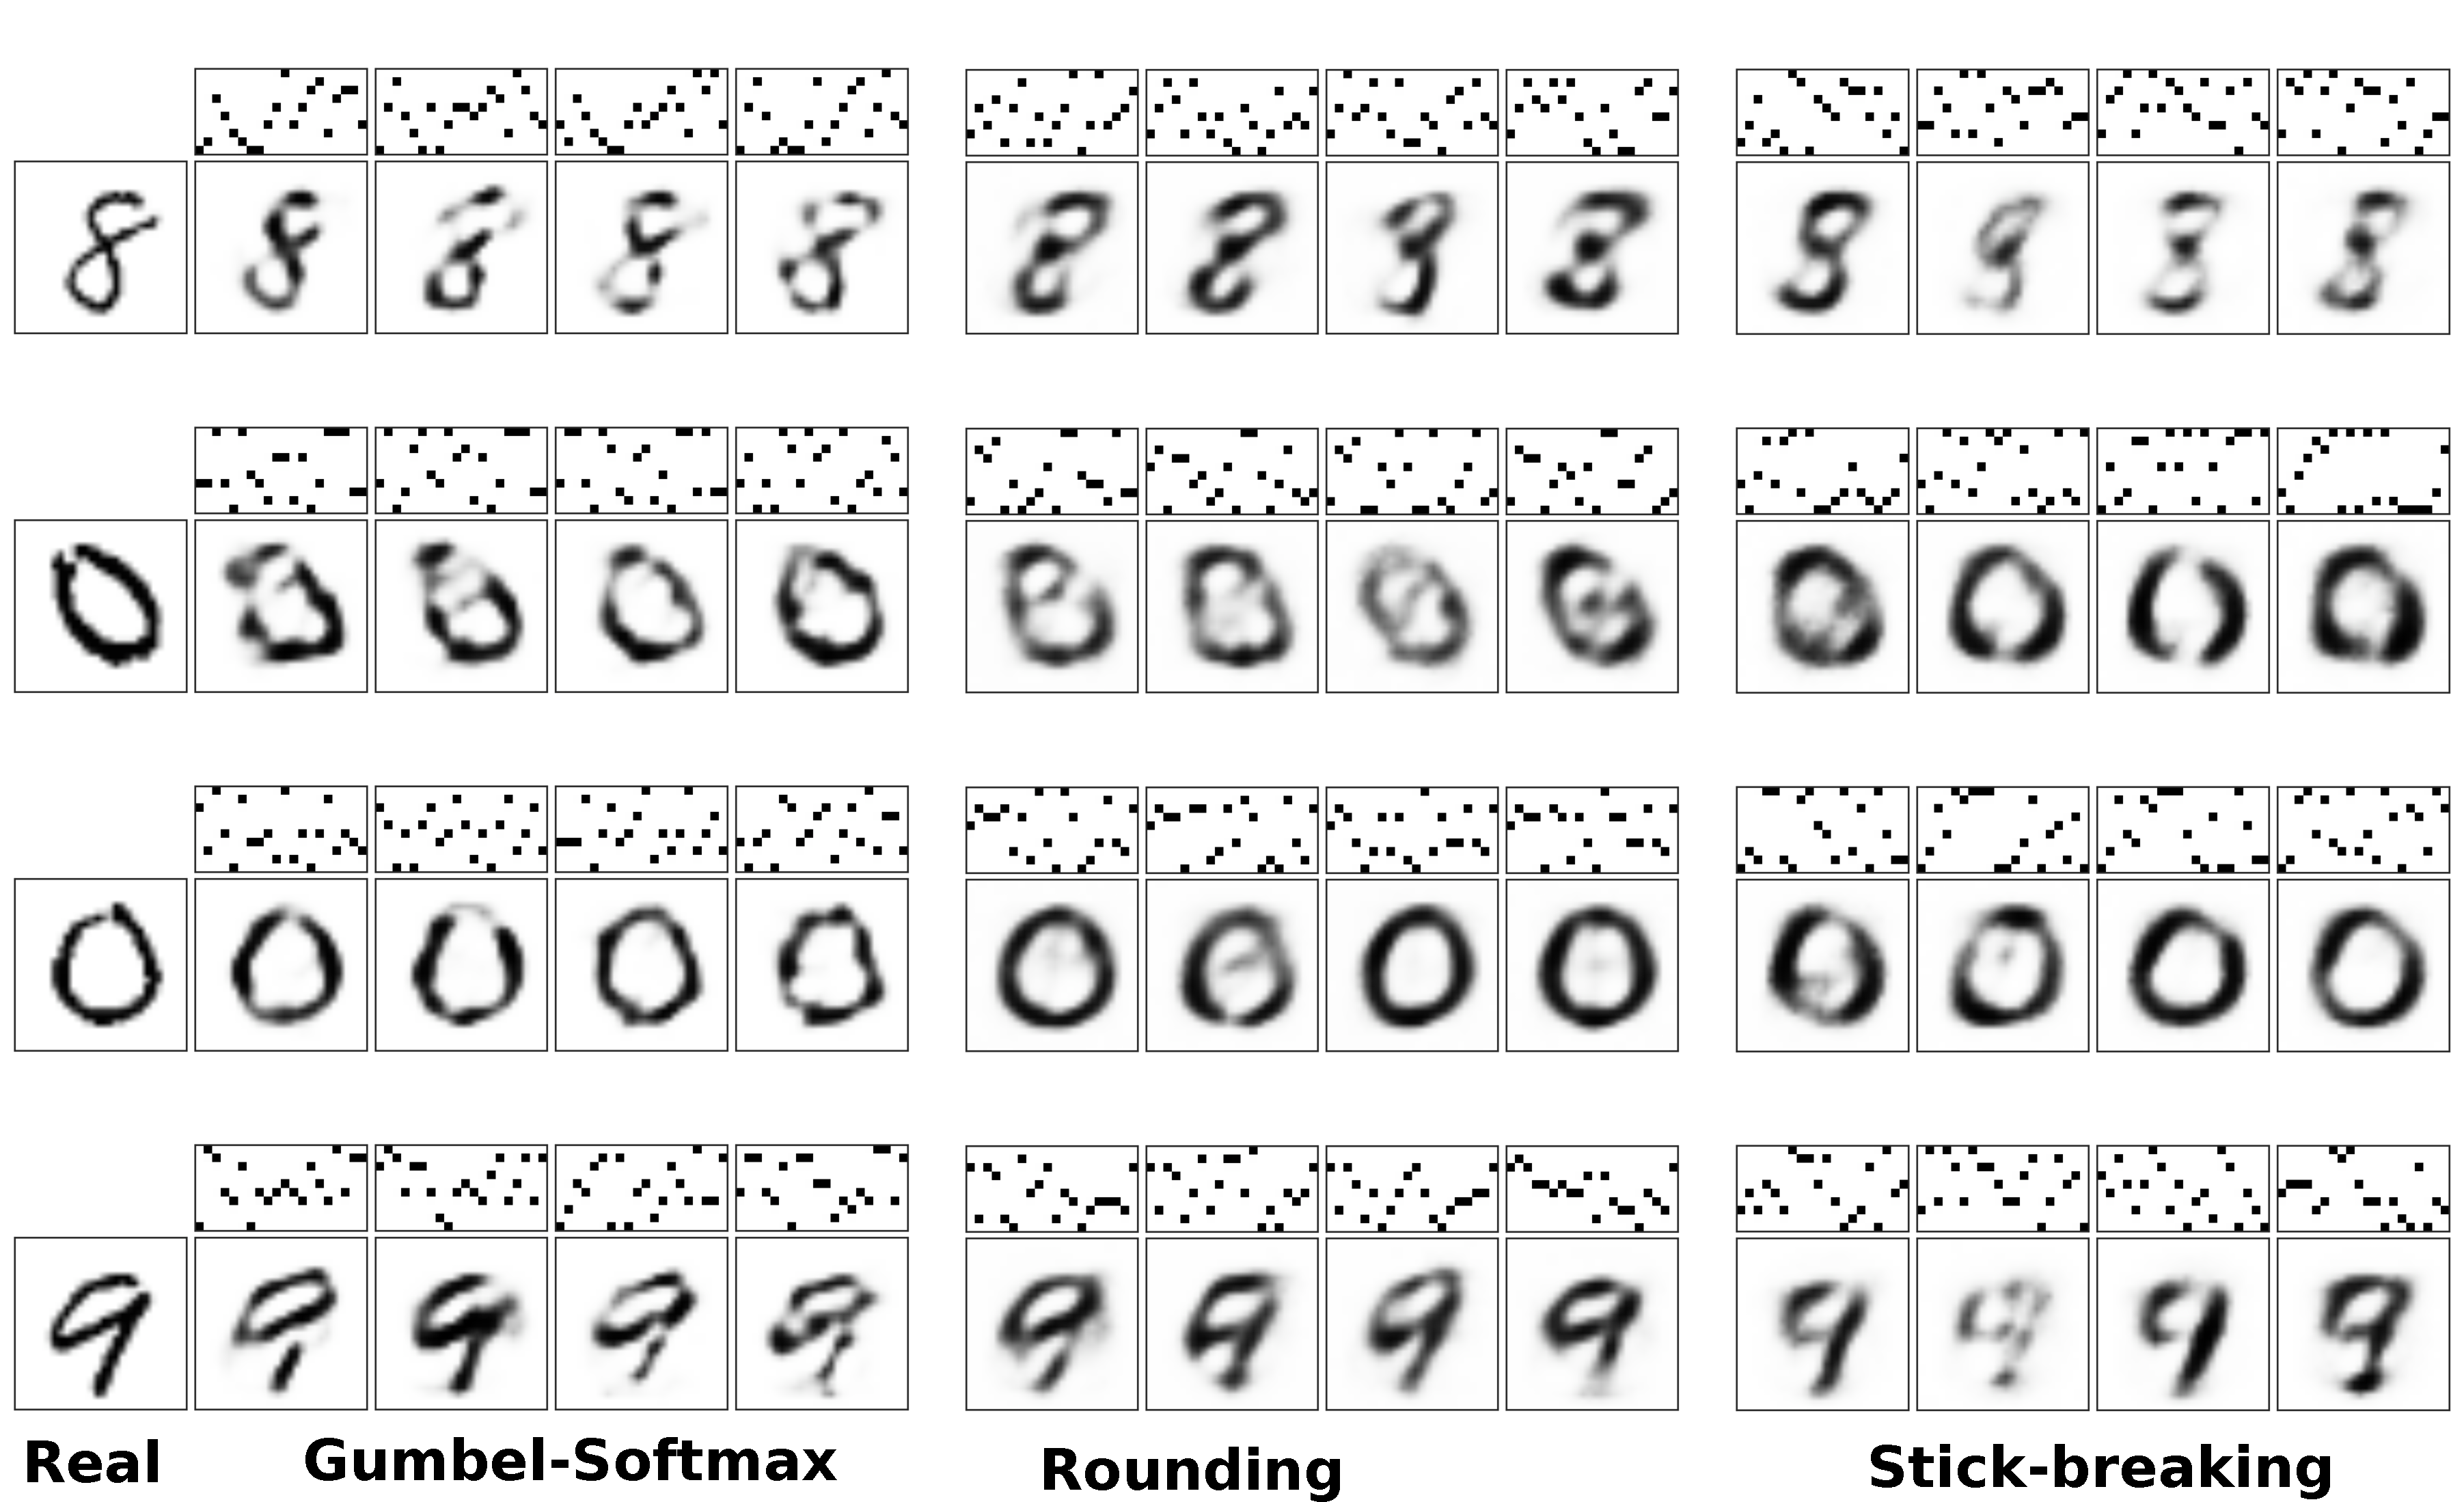
\includegraphics[width=5.in]{../figures/figure4.pdf} 
  \caption{Examples of true and reconstructed digits from their corresponding random codes using with $K=20$ categorical variables with $N=10$ possible values.
  }
\label{fig:VAE}
\end{figure*}


\section{Variational permutation inference details}

Here we discuss more of the subtleties of variational permutation
inference and present the mathematical derivations in more detail. 

\subsection{Continuous prior distributions.} 
Continuous relaxations require re-thinking the objective. As in
\cite{maddison2016concrete}, we maximize a relaxed ELBO, for which we
need to specify a new continuous prior $p(X)$ over the relaxed
discrete latent variables, here, over relaxations of permutation
matrices. Moreover, it is critical to design sensible priors for
relaxed permutations.  Ideally, this prior should penalize values
of~$X$ that are far from permutation matrices.

For our categorical experiment on MNIST we use a mixture of Gaussians
around each
vertex,~${p(x) = \tfrac{1}{N} \sum_{n=1}^N \mathcal{N}(x \given e_k,
  \eta^2)}$.  This can be extended to permutations, where use a
mixture of Gaussians for each dimension,
\begin{align}
\label{eq:permprior}
  \nonumber p(X) &= \prod_{m=1}^N \prod_{n=1}^N
  \frac{1}{2} \left(\mathcal{N}(x_{mn} \given 0, \eta^2) + \distNormal(x_{mn} \given 1, \eta^2 \right).
  \end{align}
Although this prior puts significant mass around invalid points
(e.g.~$\bone$), it penalizes $X$ that far from~$\mcB_N$.

\subsection{Deriving an expression for the ELBO}
Here we show that if $X=g(\Xi;\theta)$ with $g$ differentiable one can
evaluate the second term in equation \eqref{eq:elbo}.  Moreover, both
the stick-breaking and rounding transformations factor as
${g=h \circ f}$ with ${X = h(\Psi)}$ and ${\Psi = f(\Xi; \theta)}$.
(Both $h$ and $f$ are invertible.) This means all dependency of $X$ in
the parameters is through the random variable~$\Psi$ with implicit
density~$p(\Psi; \theta)$.

We compute the entropy of~$q(X; \theta)$ (the second term in the ELBO)
by,

\begin{align*}
  \E_{q(X; \theta)} \left[- \log q(X; \theta) \right]
  &=
    \E_{r(\Xi)} \left[- \log q(h(f(\Xi,\theta)); \theta) \right] \\
  &= \E_{p(\Psi;\theta)} \left[- \log q(h(\psi); \theta) \right]. 
\end{align*}
where the second equality follows by the ``law of the unconscious statistician.''

Now, by the change of variable theorem and derivative and determinant
inversion rules,
\begin{align*}
  q(X; \theta)
  &= p(h^{-1}(X) ;\theta) \,
    \left| \frac{\mathrm{d} h^{-1}(X)}{\mathrm{d}X} \right| \\
  &= p(h^{-1}(X); \theta)
    \left| \frac{\mathrm{d}h(\Psi)}{\mathrm{d}\Psi} \right|^{-1}_{\Psi = h^{-1}(X)}.
 \end{align*}
Now we appeal once more to the law of the unconcious statistician,
\begin{align*}
  \E_{q(X; \theta)}& \left[- \log q(X; \theta) \right] \\
  &= \E_{p(\Psi;\theta)} \left[ - \log p(\Psi;\theta) +
     \log \left| \frac{\mathrm{d} h(\Psi)}{\mathrm{d}\Psi} \right| \right] \\
  &= \bbH(\Psi; \theta)  +
  \E_{r(\Xi)}\left[\left| \frac{\mathrm{d}h(\Psi; \theta)}{\mathrm{d}\Psi} \right|_{\Psi = f(\Xi; \theta)} \right].
\end{align*}
 

\subsubsection*{Estimating the ELBO} 
Here we describe how to compute each of terms of equation \eqref{eq:elbo2}, needed for ELBO computations. First, as $\Psi$ is Gaussian for both rounding and stick-breaking, the entropy term is straightforward and equal to $N\log(\eta^2 2\pi e )/2$ ($\eta$ may depend on the temperature and depends on the method). 

Notice that to state $\Psi$ is Gaussian in the stick-breaking case we slightly deviate from \ref{sec:permutation}. Specifically, here we call $\Psi=\frac{\mu_{mn} + \eta_{mn} \Xi_{mn}}{\tau} $ and define $\Psi' = \sigma(\Psi)$.

The second term of equation \eqref{eq:elbo2} is estimated using Monte-Carlo samples, and its derivation depends on the method. 

\textbf{Rounding}

Here $H$ is piecewise linear: the set of discontinuities (border of the 'Voronoi cells' associated to each permutation) has Lebesgue measure zero. So we can still apply the change of variables theorem. Therefore, 
$\log |DH(F(\Xi;\theta)) |= N\log
\tau$. This means we don't even need to take samples to compute this term.


\textbf{Stick-breaking}

It is important to note that the transformation $H$ that maps $\Psi'\rightarrow X$ is only piecewise
continuous: the function is not differentiable at the points where
the bounds change; for example, when changing~$\Psi'$ causes the
active upper bound to switch from the row to the column constraint
or vice versa.  

Notice that these bounds only depend on values of~$X$ that
have already been computed; i.e., those that are above or to the left of
the~$(i,j)$-th entry. Thus, the transformation from ~$\Psi'$ to~$X$
is feed-forward according to this ordering.  Consequently, the
Jacobian of the inverse transformation $H^{-1}$ ,~$\mathrm{d}\Psi' / \mathrm{d} X$,
is lower triangular, and its determinant is the product of its diagonal,
\begin{align}
\nonumber \left| \frac{\mathrm{d} \Psi'} {\mathrm{d} X} \right|
&= \prod_{i=1}^{n-1} \prod_{j=1}^{n-1} \frac{\partial \psi_{ij} }{\partial {\pi}_{ij}} \\
\nonumber &= \prod_{i=1}^{n-1} \prod_{j=1}^{n-1} \frac{\partial}{\partial {\pi}_{ij}}
\sigma^{-1} \left( \frac{{\pi}_{ij} - \ell_{ij}}{u_{ij} - \ell_{ij}} \right ) \\
\nonumber &= \prod_{i=1}^{n-1} \prod_{j=1}^{n-1}
\left( \frac{1}{u_{ij} - \ell_{ij}} \right )
\left( \frac{u_{ij} - \ell_{ij}}{{\pi}_{ij} - \ell_{ij}} \right )
\left( \frac{u_{ij} - \ell_{ij}}{u_{ij} - {\pi}_{ij}} \right ) \\
\nonumber &= \prod_{i=1}^{n-1} \prod_{j=1}^{n-1}
\frac{u_{ij} - \ell_{ij}}{({\pi}_{ij} - \ell_{ij}) (u_{ij} - {\pi}_{ij})}
\end{align}

To compute the gradient of the forward transformation $H$ one simply needs to invert the above (or put a negative sign, in the logarithm scale). Finally,  to incorporate the effect of $\sigma$ ($\Psi'=\sigma(\Psi)$, by the chain rule,  one only needs to add a term corresponding to this derivative, $d\sigma(x)/dx=\sigma(x)\sigma(-x)$. 
\subsection*{Experiment details}

Experiments were run on a High Performance Computing (HPC) cluster, allowing the execution of hundreds of processes in parallel to efficiently determine best hyperparameter configurations.

For experiments with Variational Auto-encoder we used Tensorflow \citep{Abadi2016}, slightly changing the code made available in conjunction with \cite{Jang2016}. For experiments on synthetic matching and the C. elegans example we used Autograd  \citep{maclaurin2015autograd}, explicitly avoiding propagating gradients through the non-differentiable operation of solving a matching problem (the $\mathsf{round}$ in \ref{sub:rounding}).

In all experiment we used the ADAM as optimizer, with learning rate 0.1. For rounding, the parameter vector $H$ defined in \ref{sub:rounding}(iii) was constrained to lie in the interval $[0.1, 0.5]$. Also, for rounding, we used ten iterations of the Sinkhorn-Knopp algorithm, to obtain points in the Birkhoff polytope. For stick-breaking the variances $\nu$ defined in \ref{sub:stickbreaking} was constrained between $1e-8$ and 1.0. In either case, the temperature parameter was calibrated using a grid search.
 
In the C. elegans example we considered the symmetrized version of the adjacency matrix described in \citep{varshney2011structural} (i.e. we used $A'=(A+A^\top)/2$, and the matrix $W$ was chosen antisymmetric, with entries sampled randomly with the sparsity pattern dictated by $A'$. To avoid divergence, the matrix $W$ was then re-scaled by 1.1 times its spectral radius. This choice, although not essential, induced a reasonably well behaved linear dynamical system, rich in non-damped oscillations. We used a time window of $T=1000$ time samples, and added spherical standard noise at each time 


\bibliography{refs}
\bibliographystyle{abbrvnat}


\end{document}
